\begin{frame}{Manipulator Description}
    \begin{columns}
        \begin{column}{.75\linewidth}
            The Manipulator Description comes from the \href{https://github.com/UniversalRobots/Universal_Robots_ROS2_Description/tree/humble}{``Humble'' branch of the official GitHub repository}.

            Several modifications were made to the original URDF to allow for the Gazebo Simulation and inclusion of a Depth Camera and Gripper.
        \end{column}
        \begin{column}{.25\linewidth}
            \begin{center}
                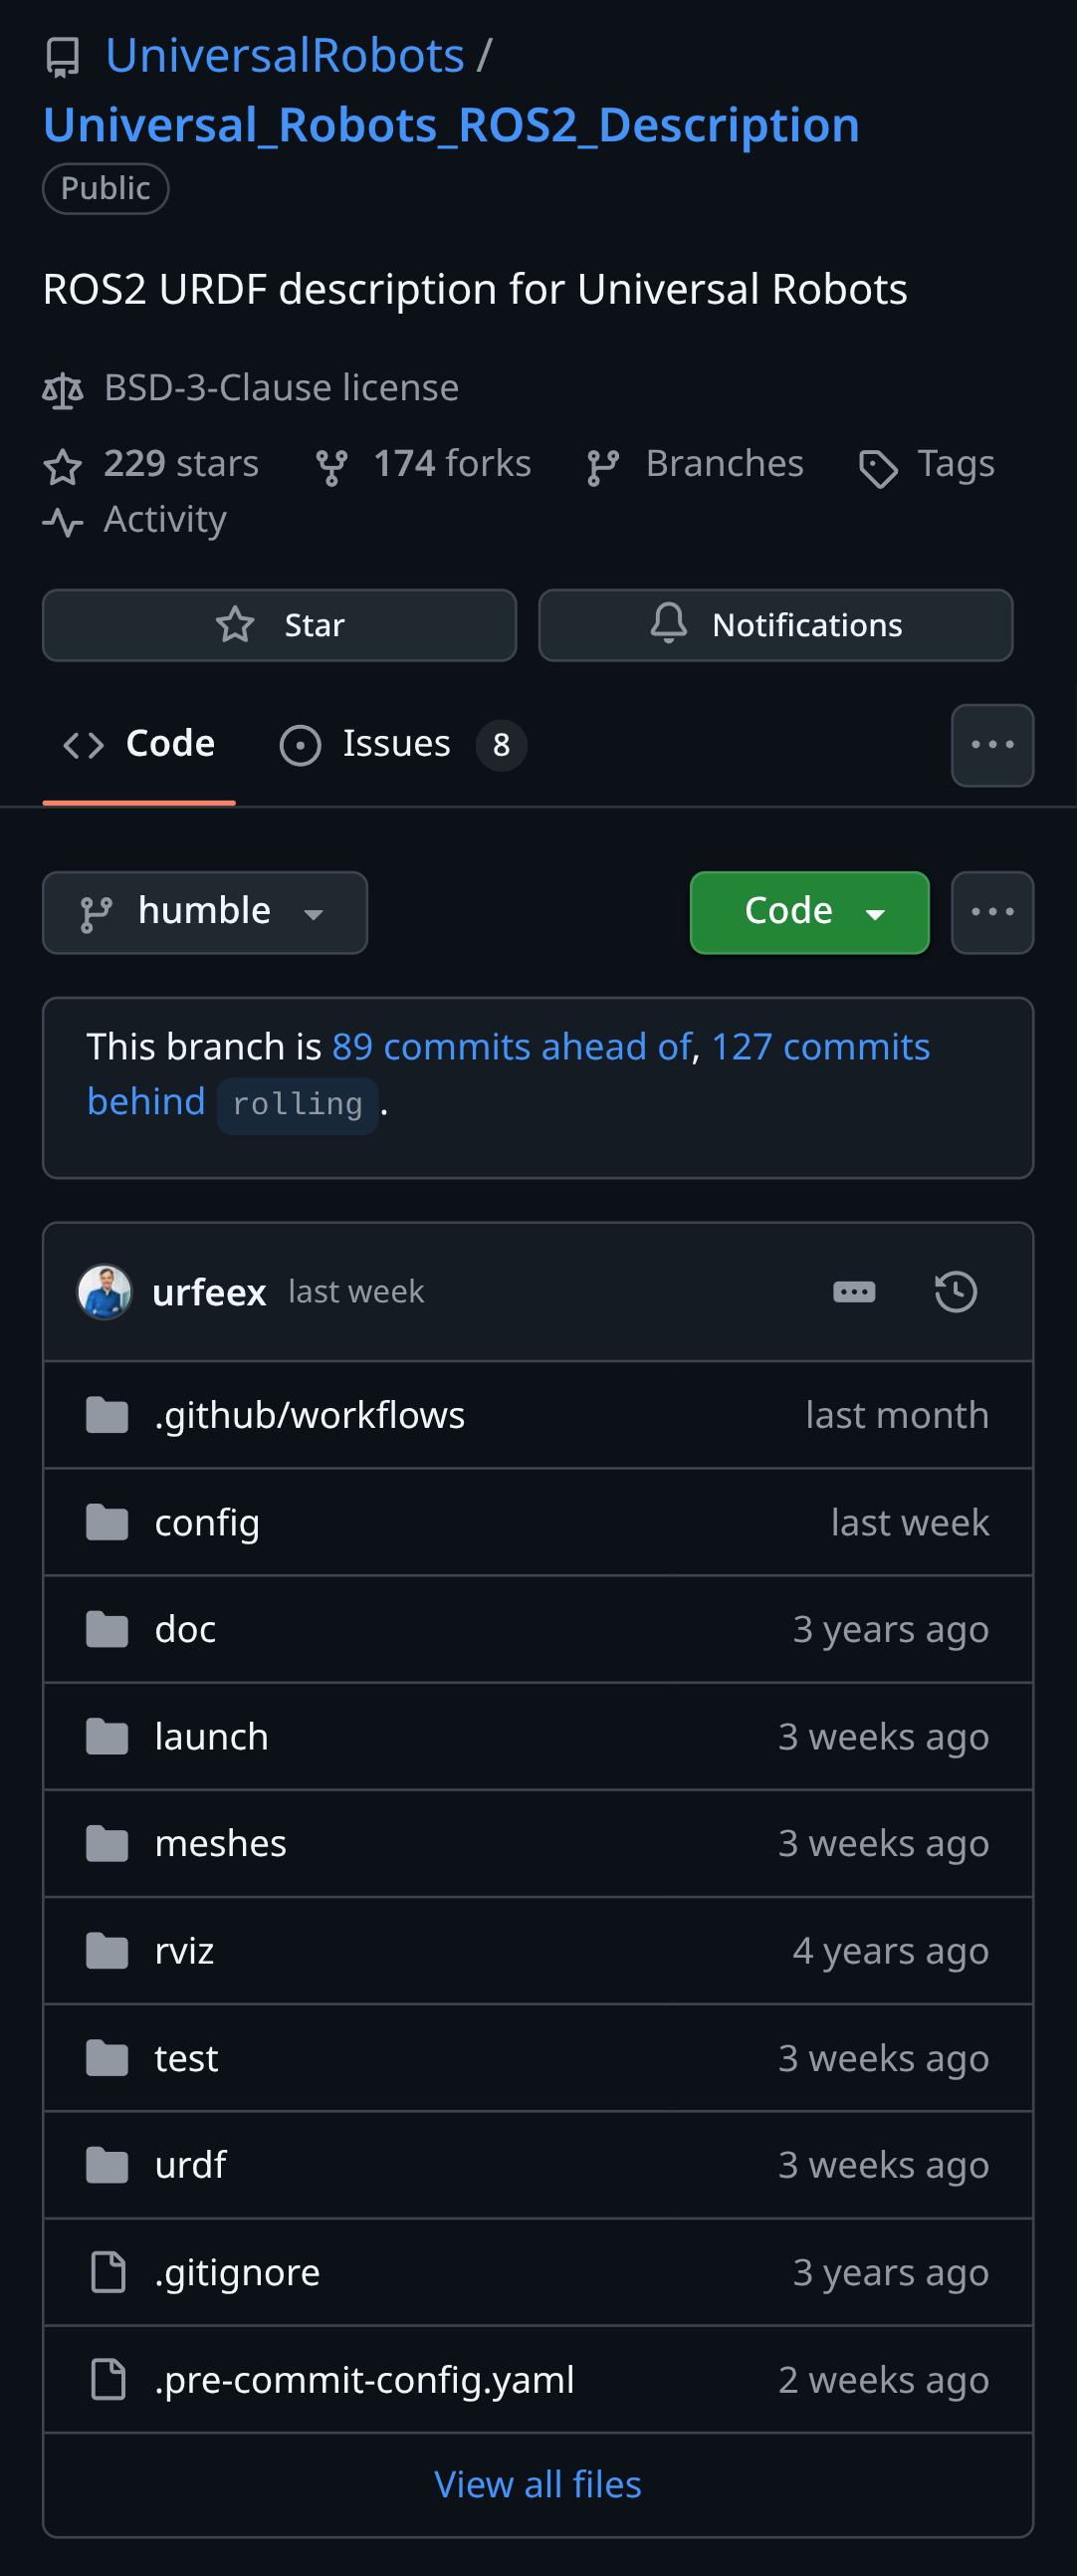
\includegraphics[width=.75\textwidth]{media/UR5DescriptionRepo.png}
            \end{center}
        \end{column}
    \end{columns}
\end{frame}
\begin{frame}{Gripper Description}
    \begin{columns}
        \begin{column}{.75\linewidth}
            The Robotiq 2f85 Gripper Description comes from the \href{https://github.com/PickNikRobotics/ros2_robotiq_gripper/tree/humble}{``Humble'' branch of the PickNikRobotics' GitHub repository}.

            Several modifications were made to the original URDF to allow for the Gazebo Simulation, which was initially not supported.
        \end{column}
        \begin{column}{.25\linewidth}
            \begin{center}
                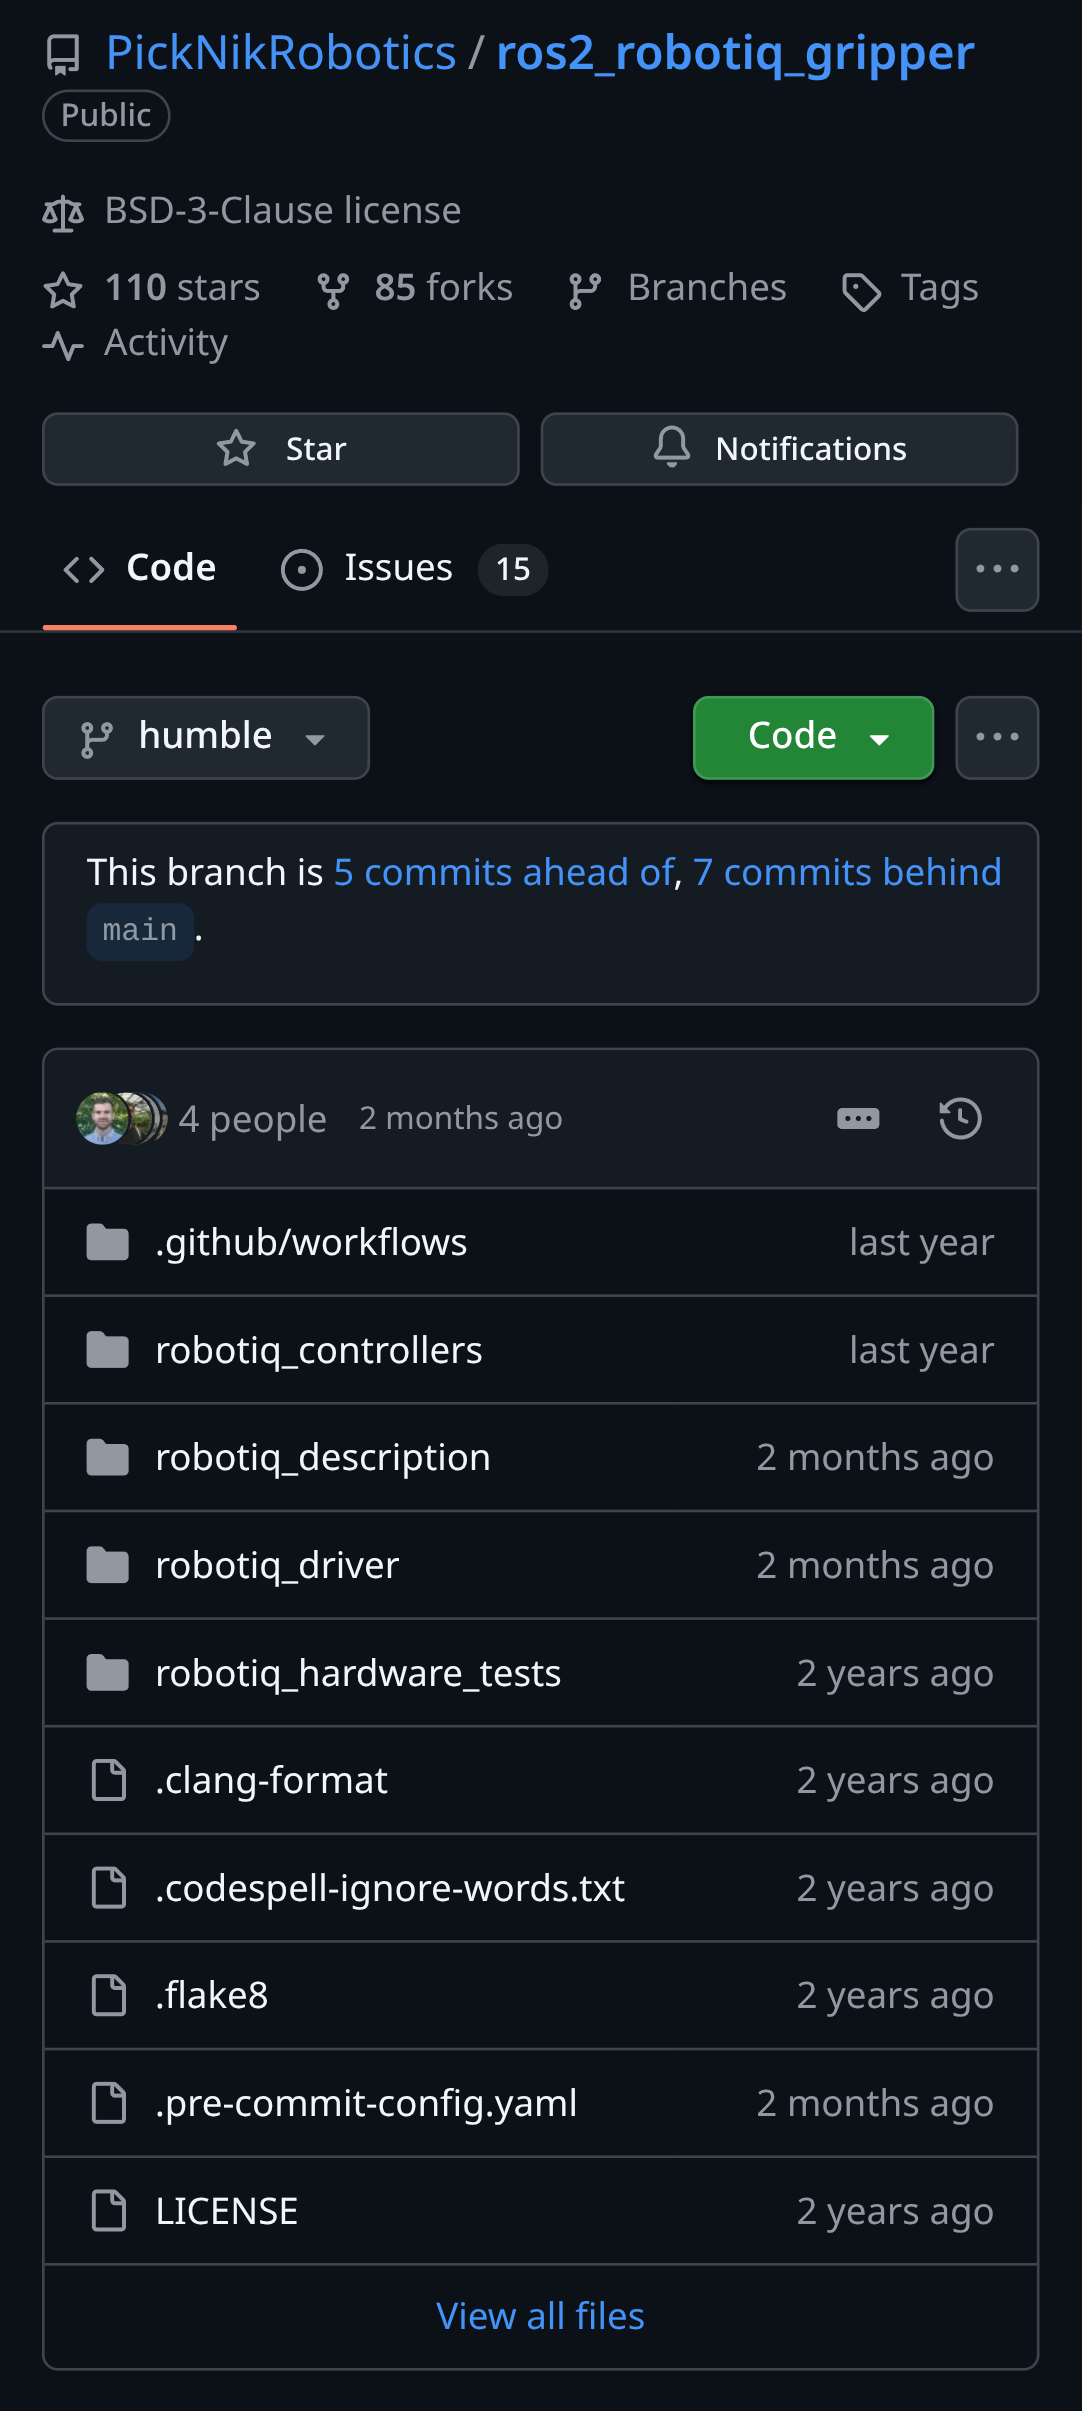
\includegraphics[width=.75\textwidth]{media/RobotiqGripperDescriptionRepo.png}
            \end{center}
        \end{column}
    \end{columns}
\end{frame}
\begin{frame}{Robot Controllers}
    The controllers used were the ones from the description repositories, grouped in a single file for ease of use.

    This means that the MoveIt2 dummy controllers were to be replaced in the final MoveIt Configuration Package.

    Especially the Joint Trajectory Controller and the Gripper Action Controller were useful for the project purposes.
\end{frame}
\begin{frame}{Depth Camera Description}
    The Depth camera is entirely simulated:
    \begin{itemize}
        \item $1024px \times 768px$ Resolution
        \item $2.24\mu m \times 2.24\mu m$ pixels
        \item Minimum perceived depth of $0.10 m$
        \item Maximum perceived depth of $2.25 m$
    \end{itemize}
    It is positioned $2m$ above and $50cm$ in front of the Base Link of the Robot, while pointing down.
\end{frame}
\begin{frame}{Gazebo World}
    \begin{columns}
        \begin{column}{.5\linewidth}
            The world consists in three objects:
            \begin{itemize}
                \item Robot Base
                \item Target Base
                \item Target
            \end{itemize}
        \end{column}
        \begin{column}{.5\linewidth}
            \begin{center}
                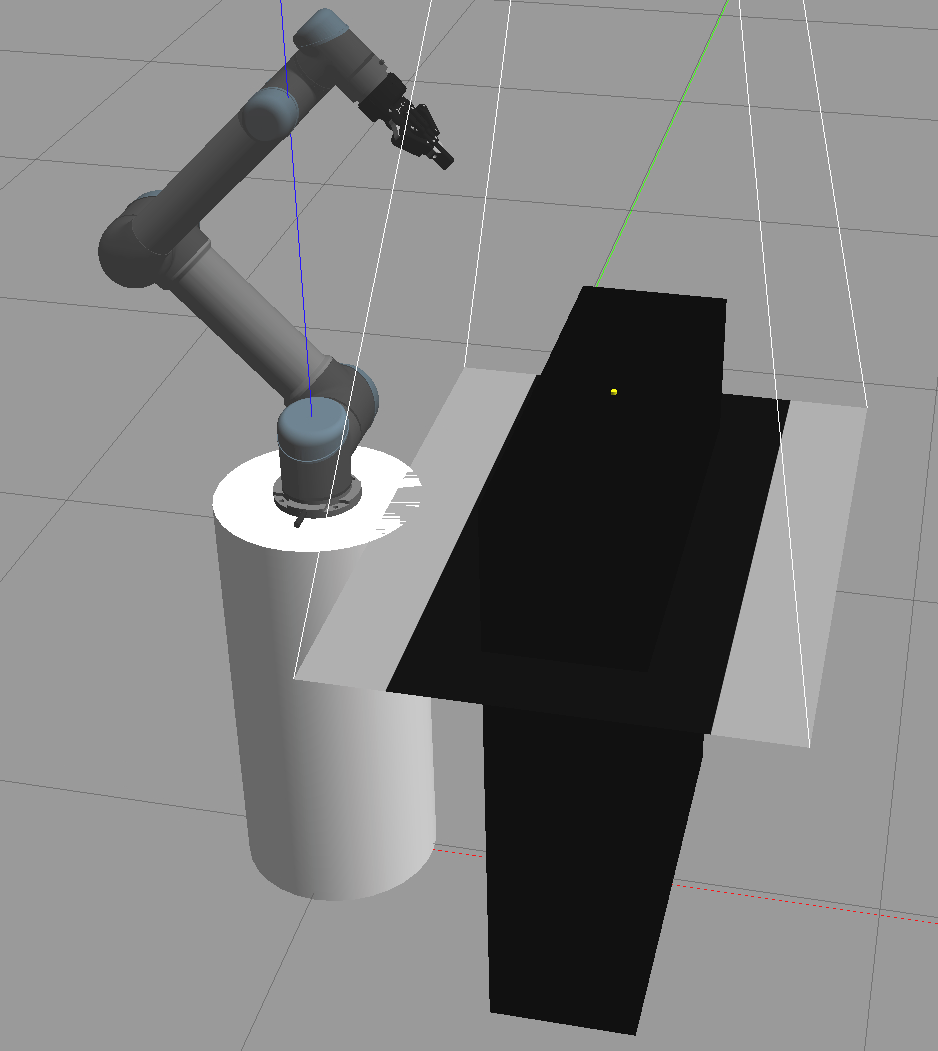
\includegraphics[width=.75\textwidth]{media/GazeboWorld.png}
            \end{center}
        \end{column}
    \end{columns}
\end{frame}
\begin{frame}{MoveIt Setup - Move Groups and Controllers}
    Two move groups:
    \begin{enumerate}
        \item ``\texttt{ur\textunderscore manipulator}'' $\rightarrow$ The UR5 Manipulator
        \item ``\texttt{ur\textunderscore gripper}'' $\rightarrow$ The Robotiq 2f85 Gripper
    \end{enumerate}
    Two ROS2 controllers:
    \begin{enumerate}
        \item ``\texttt{joint\textunderscore trajectory\textunderscore controller}'' $\rightarrow$ \texttt{JointTrajectoryController}
        \item ``\texttt{gripper\textunderscore position\textunderscore controller}'' $\rightarrow$ \texttt{GripperActionController}
    \end{enumerate}
    Two MoveIt2 controllers:
    \begin{enumerate}
        \item ``\texttt{joint\textunderscore trajectory\textunderscore controller}'' $\rightarrow$ \texttt{FollowJointTrajectory}
        \item ``\texttt{gripper\textunderscore position\textunderscore controller}'' $\rightarrow$ \texttt{GripperCommand}
    \end{enumerate}
\end{frame}
\begin{frame}{MoveIt Setup - Motion Planners}
    Adapted using the correct move groups from the MoveIt2 tutorials repository:
    \begin{itemize}
        \item ``\texttt{chomp\textunderscore planning.yaml}''
        \item ``\texttt{lerp\textunderscore planning.yaml}''
        \item ``\texttt{ompl\textunderscore planning.yaml}''
        \item ``\texttt{pilz\textunderscore industrial\textunderscore motion\textunderscore planner\textunderscore planning.yaml}''
        \item ``\texttt{trajopt\textunderscore planning.yaml}''
    \end{itemize}
\end{frame}
\begin{frame}{Running the Inverse Kinematics}
    \begin{columns}
        \begin{column}{.5\linewidth}
            The Inverse Kinematics is ran using the MoveIt2 APIs in a C++ ROS2 node.
        \end{column}
        \begin{column}{.5\linewidth}
            \inputminted[
                fontsize=\tiny,
                breaklines,
                firstline=174,
                lastline=180
            ]{c++}{../ros-humble-sim_workspace/ws_ur/src/ur_gripper_sim/src/run_ik.cpp}   
        \end{column}
    \end{columns}
\end{frame}
\begin{frame}{Running the Inverse Kinematics}
    \begin{columns}
        \begin{column}{.25\linewidth}
            The world objects geometries are added to the planning scene for the Motion Planner to avoid them.
        \end{column}
        \begin{column}{.75\linewidth}
            \inputminted[
                fontsize=\tiny,
                breaklines,
                firstline=190,
                lastline=213
            ]{c++}{../ros-humble-sim_workspace/ws_ur/src/ur_gripper_sim/src/run_ik.cpp}   
        \end{column}
    \end{columns}
\end{frame}
\begin{frame}{Running the Inverse Kinematics}
    \begin{columns}
        \begin{column}{.35\linewidth}
            The object contours coordinates are loaded into a ``\texttt{pts}'' vector, and the waypoints are computed by combining such coordinates and a predefined target orientation.
        \end{column}
        \begin{column}{.65\linewidth}
            \inputminted[
                fontsize=\tiny,
                breaklines,
                firstline=233,
                lastline=236
            ]{c++}{../ros-humble-sim_workspace/ws_ur/src/ur_gripper_sim/src/run_ik.cpp}
            \inputminted[
                fontsize=\tiny,
                breaklines,
                firstline=238,
                lastline=239
            ]{c++}{../ros-humble-sim_workspace/ws_ur/src/ur_gripper_sim/src/run_ik.cpp}
            \inputminted[
                fontsize=\tiny,
                breaklines,
                firstline=242,
                lastline=252
            ]{c++}{../ros-humble-sim_workspace/ws_ur/src/ur_gripper_sim/src/run_ik.cpp}
        \end{column}
    \end{columns}
\end{frame}
\begin{frame}{Running the Inverse Kinematics}
    \begin{columns}
        \begin{column}{.35\linewidth}
            Finally, a cartesian path is computed and the trajectory with its timing law is executed.
        \end{column}
        \begin{column}{.65\linewidth}
            \inputminted[
                fontsize=\tiny,
                breaklines,
                firstline=254,
                lastline=265
            ]{c++}{../ros-humble-sim_workspace/ws_ur/src/ur_gripper_sim/src/run_ik.cpp}
            \inputminted[
                fontsize=\tiny,
                breaklines,
                firstline=267,
                lastline=269
            ]{c++}{../ros-humble-sim_workspace/ws_ur/src/ur_gripper_sim/src/run_ik.cpp}
        \end{column}
    \end{columns}
\end{frame}